\documentclass{standalone}
\usepackage{tikz}
\usepackage{ctex}
\setCJKmainfont{Noto Serif CJK SC}
\usepackage{chemmacros,siunitx}
\usetikzlibrary{patterns, calc}
\usetikzlibrary {decorations.pathmorphing, decorations.pathreplacing, decorations.shapes}
\begin{document}
\small
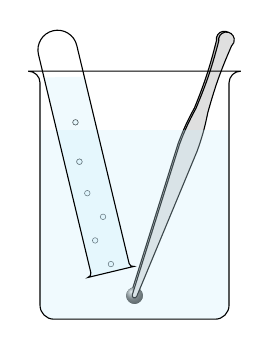
\begin{tikzpicture}[>=latex,scale=1.0]
  \begin{scope}[yshift=0.3cm,rotate=-20]
    \draw[fill=lightgray](-0.05,0)--(-0.14,2)to[bend left=4](-0.1,2.5)to[bend right=4](-0.13,3.4)arc(210:-30:0.1);
    \fill[ball color=gray](0,0)circle(3pt);
    \draw[fill=lightgray!50](-0.03,0)--(-0.12,2)to[bend left=4](-0.08,2.5)to[bend right=4](-0.1,3.4)arc(210:-30:0.1)to[bend right=4](0.08,2.5)to[bend left=4](0.12,2)--(0.03,0)arc(360:180:0.03);
  \end{scope}
  \foreach \x/\y in {
    -0.3/0.7,
    -0.5/1.0,
    -0.4/1.3,
    -0.6/1.6,
    -0.7/2.0,
    -0.7/2.0,
    -0.75/2.5}
  {
    \draw[very thin,fill=cyan!5!white](\x,\y)circle(1pt);
  }
  \fill[cyan!20!white,opacity=0.3,rounded corners=5pt](-1.2,2.4)--(-1.2,0)--(1.2,0)--(1.2,2.4);
  \draw[rounded corners=5pt](-1.2,3.0)--(-1.2,0)--(1.2,0)[sharp corners]--(1.2,3.0)arc(180:90:0.15)--++(-2.7,0)arc(90:0:0.15);
  \begin{scope}[xshift=-0.3cm,yshift=0.6cm,rotate=13.5]
    \fill[cyan!20!white,opacity=0.3](-0.30,0)arc(-90:0:0.05)--(-0.25,2.6)--(0.25,2.49)--(0.25,0.05)arc(180:270:0.05)--cycle;
    \draw(-0.30,0)arc(-90:0:0.05)--(-0.25,2.9)arc(180:0:0.25)--(0.25,0.05)arc(180:270:0.05)--cycle;
  \end{scope}
\end{tikzpicture}
\end{document}